\chapter{Trainer Kit Emulator}

The keyboard enables the user to enter and store the 8085 Hex machine code in the R/W memory. The seven segment display is used to display memory addresses and their contents while entering , monitoring or modifying the programs. It also has two LEDS which blink alternatively on program execution. The Graphical Trainer Kit can be launched from the sub-menu item ``\textbf{8085 microprocessor trainer kit}'' placed under menu item ``View''. Shortcut key for launching this Trainer Kit Emulator is \textbf{"F9"}. 
In the back-end it is basically using the same engine, so at any step user can switch between any two environments.

\begin{figure}[htbp]
\centering
\includegraphics[width=0.75\linewidth]{"./kit"}
\caption{8085 Trainer Kit}
\end{figure}

\section{Keyboard}
The keyboard has 24 keys; 16 keys for the Hex digits 0 to F and remaining keys are used to perform various functions. Some of the Hex digit keys has dual function: data entry mode and register monitor mode. The function of these keys are described as follows:

\begin{enumerate}
\item 0 to F: Enter Hex digits
\item Reset: To terminate the current execution. It does not clear register or memory contents. It is doing the same function as pressing STOP button during the execution of code in 8085 simulator workspace. To clear memory content, goto Settings $ \rightarrow $ Clear Memory, or press "CTRL+SHIFT+DELETE".  
\item Halt: It pauses the program at any stage of execution. It is equivalent to pressing PAUSE during the execution of code in 8085 simulator workspace. From where it is possible to do both forward and backward traversal.
\item DCR: Decrements the memory address and displays the new address and its data.
\item INR: Increments the memory address and displays the new address and its data.
\item SET/MEM: To enter contents in particular memory address.
\item REG: To monitor the current register content.
\item GO: To set the starting address of execution.
\item EXEC: To begin execution of the program from the begin address that is set. It takes the simulation speed that is default by the user in the editor. But, the default speed is set to ultimate. 
\end{enumerate}

\section{Using the Trainer Kit Emulator}

\subsection{How to enter a program}
Let's take one of the sample program as shown in \cref{fig:samplecode2}, to illustrate the programing process. The detailed step by step loading instruction are given in \cref{table:trainer:load}.
\begin{figure}[htbp]
\centering
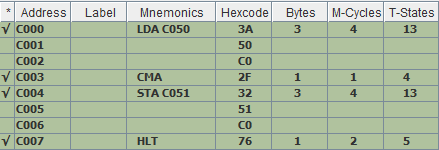
\includegraphics[width=0.75\linewidth]{sampleCode2Asm}
\caption{Sample Program of 1's COMPLEMENT OF AN 8-BIT NUMBER}
\label{fig:samplecode2}
\end{figure}

When we load a program we enter the Hex codes in memory locations for given instructions.\\

{
\begin{table}[htbp]
\caption{Showing the buttons to be pressed sequentially to load the program in the memory}
\label{table:trainer:load}
\centering
\newcommand\Ts{\rule{0pt}{2.6ex}}       % top strut
\newcommand\Bs{\rule[-1.1ex]{0pt}{0pt}} % bottom strut
\begin{tabular}{lrc}
\toprule
\multicolumn{3}{c}{To load the Program}\\
\midrule
STEP & 1: & \boxed{RESET}\\
STEP &  2: & \Ts\boxed{SET/MEM}\Bs\\
STEP &  3: & \Ts\boxed{C} \boxed{0} \boxed{0} \boxed{0}\Bs\\
STEP &  4: & \Ts\boxed{INR}\Bs\\
STEP &  5: & \Ts\boxed{3} \boxed{A}\Bs\\
STEP &  6: & \Ts\boxed{INR}\Bs\\
STEP &  7: & \Ts\boxed{5} \boxed{0}\Bs\\
STEP &  8: & \Ts\boxed{INR}\Bs\\
STEP &  9: & \Ts\boxed{C} \boxed{0}\Bs\\
STEP & 10: & \Ts\boxed{INR}\Bs\\
STEP & 11: & \Ts\boxed{2} \boxed{F}\Bs\\
STEP & 12: & \Ts\boxed{INR}\Bs\\
STEP & 13: & \Ts\boxed{3} \boxed{2}\Bs\\
STEP & 14: & \Ts\boxed{INR}\Bs\\
STEP & 15: & \Ts\boxed{5} \boxed{1}\Bs\\
STEP & 16: & \Ts\boxed{INR}\Bs\\
STEP & 17: & \Ts\boxed{C} \boxed{0}\Bs\\
STEP & 18: & \Ts\boxed{INR}\Bs\\
STEP & 19: & \Ts\boxed{7} \boxed{6}\Bs\\
\midrule
\multicolumn{3}{c}{To load a value in C050}\\
\midrule
STEP & 20: & \Ts\boxed{SET/MEM}\Bs\\
STEP & 21: & \Ts\boxed{C} \boxed{0} \boxed{5} \boxed{0}\Bs\\
STEP & 22: & \Ts\boxed{INR}\Bs\\
STEP & 23: & \Ts\boxed{9} \boxed{6}\Bs\\
\bottomrule
\end{tabular}
\end{table}
}

\subsection{To Execute the Program}
For proper execution of the program, it is needed to direct the processor to the starting address of the code and then begin execution, as shown in \cref{table:trainer:exec}.

{
\begin{table}[htbp]
\caption{Showing the buttons to be pressed for proper execution of the code}
\label{table:trainer:exec}
\centering
\newcommand\Ts{\rule{0pt}{2.6ex}}       % top strut
\newcommand\Bs{\rule[-1.1ex]{0pt}{0pt}} % bottom strut
\begin{tabular}{lrc}
\toprule
\multicolumn{3}{c}{To begin execution}\\
\midrule
STEP & 1: & \boxed{RESET}\\
STEP &  2: & \Ts\boxed{GO}\Bs\\
STEP &  3: & \Ts\boxed{C} \boxed{0} \boxed{0} \boxed{0}\Bs\\
STEP &  4: & \Ts\boxed{EXEC}\Bs\\
\bottomrule
\end{tabular}
\end{table}
}

\subsection{How to examine memory and register contents}
After program execution it is essential to examine the contents of registers and memory. \Cref{table:trainer:monitor} lists the methods to access each and every register. It also lists how to examine the content at particular memory address.
{
\begin{table}[htbp]
\caption{Showing the buttons to be pressed for register and memory monitoring}
\label{table:trainer:monitor}
\centering
\newcommand\Ts{\rule{0pt}{2.6ex}}       % top strut
\newcommand\Bs{\rule[-1.1ex]{0pt}{0pt}} % bottom strut
\begin{tabular}{lrc}
\toprule
\multicolumn{3}{c}{To examine Accumulator}\\
\midrule
STEP & 1: & \boxed{REG}\\
STEP &  2: & \Ts\boxed{0 A}\Bs\\
\bottomrule
\toprule
\multicolumn{3}{c}{To examine B}\\
\midrule
STEP & 1: & \boxed{REG}\\
STEP &  2: & \Ts\boxed{1 B}\Bs\\
\bottomrule
\toprule
\multicolumn{3}{c}{To examine C}\\
\midrule
STEP & 1: & \boxed{REG}\\
STEP &  2: & \Ts\boxed{2 C}\Bs\\
\bottomrule
\toprule
\multicolumn{3}{c}{To examine D}\\
\midrule
STEP & 1: & \boxed{REG}\\
STEP &  2: & \Ts\boxed{3 D}\Bs\\
\bottomrule
\toprule
\multicolumn{3}{c}{To examine E}\\
\midrule
STEP & 1: & \boxed{REG}\\
STEP &  2: & \Ts\boxed{4 E}\Bs\\
\bottomrule
\toprule
\multicolumn{3}{c}{To examine H}\\
\midrule
STEP & 1: & \boxed{REG}\\
STEP &  2: & \Ts\boxed{5 H}\Bs\\
\bottomrule
\toprule
\multicolumn{3}{c}{To examine L}\\
\midrule
STEP & 1: & \boxed{REG}\\
STEP &  2: & \Ts\boxed{6 L}\Bs\\
\bottomrule
\toprule
\multicolumn{3}{c}{To examine Memory pointed by HL}\\
\midrule
STEP & 1: & \boxed{REG}\\
STEP &  2: & \Ts\boxed{7 M}\Bs\\
\bottomrule
\toprule
\multicolumn{3}{c}{To examine Stack Pointer}\\
\midrule
STEP & 1: & \boxed{SP}\\
STEP &  2: & \Ts\boxed{8 SP}\Bs\\
\bottomrule
\toprule
\multicolumn{3}{c}{To examine Program Counter}\\
\midrule
STEP & 1: & \boxed{PC}\\
STEP &  2: & \Ts\boxed{9 PC}\Bs\\
\bottomrule
\bottomrule
\toprule
\multicolumn{3}{c}{To examine a Memory Address}\\
\midrule
STEP &  1: & \Ts\boxed{SET/MEM}\Bs\\
STEP &  2: & \Ts\boxed{C} \boxed{0} \boxed{5} \boxed{1}\Bs\\
STEP & 3: & \Ts\boxed{INR}\Bs\\
\bottomrule
\end{tabular}
\end{table}
}

\section{Shortcut Keys for Trainer Kit Button}
To prevent too much switching between keyboard and mouse, some handy shortcut key listeners are integrated with some commonly used buttons, as listed in \cref{table:trainer:shortcut}.
{
\begin{table}[htbp]
\caption{List of shortcut keys}
\label{table:trainer:shortcut}
\centering
\newcommand\Ts{\rule{0pt}{2.6ex}}       % top strut
\newcommand\Bs{\rule[-1.1ex]{0pt}{0pt}} % bottom strut
\begin{tabular}{lc}
\toprule
\textbf{Keys} & \textbf{Buttons}\\
\midrule
\textbf{Esc} & RESET\\
\textbf{Alphanumeric Keys: 0-9,A-F} & HEXADECIMAL DIGITS\\
\textbf{Up-Arrow} & INR\\
\textbf{Down-Arrow} & DCR\\
\bottomrule
\end{tabular}
\end{table}
}